\documentclass{standalone}
\usepackage{tikz,times}
\usetikzlibrary{mindmap,trees,backgrounds}
\usetikzlibrary{shapes.multipart}
\begin{document}
    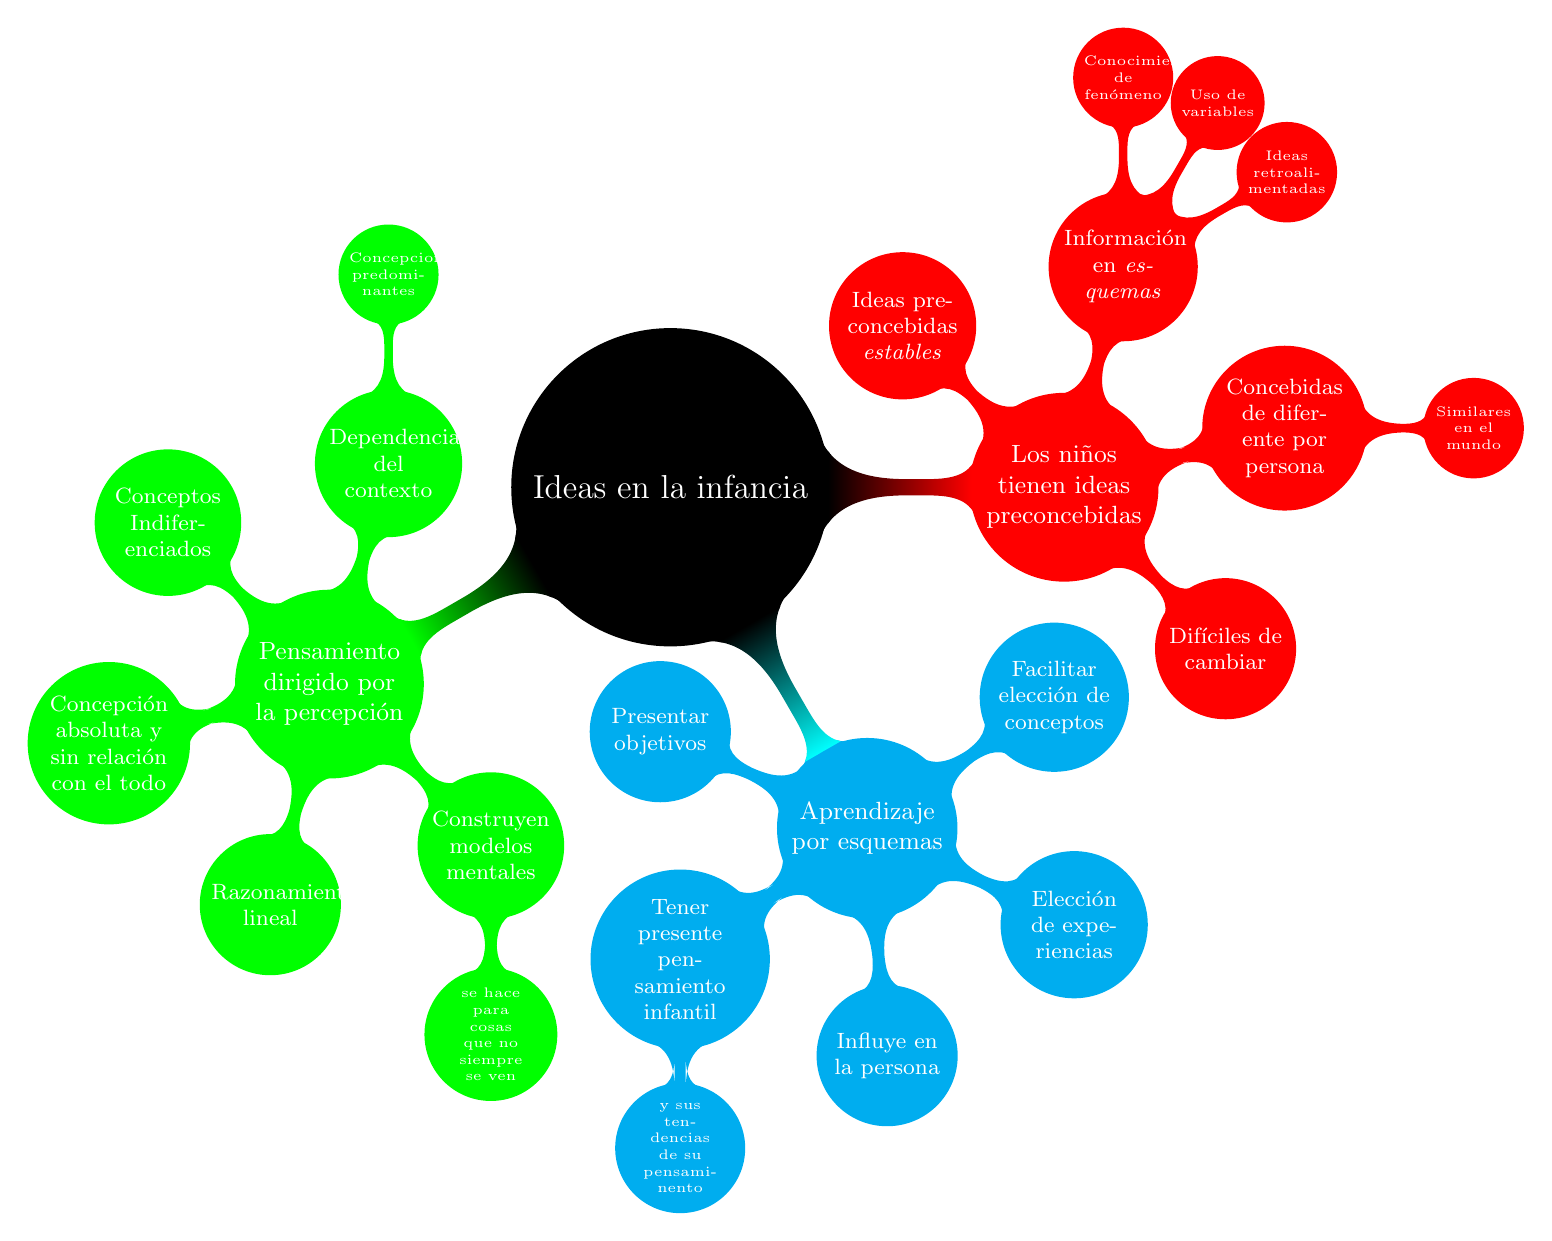
\begin{tikzpicture}
        \path[mindmap,concept color=black,text=white]
        node[concept] {Ideas en la infancia}[clockwise from=0]
        child[concept color=red] {
            node[concept]{Los niños tienen ideas preconcebidas}
            [clockwise from=135]
            child{ node[concept]{Ideas preconcebidas \textit{estables}} }
            child{ node[concept]{Información en \textit{esquemas}}
                [clockwise from=90]
                child{ node[concept]{Conocimiento de fenómeno}}
                child{ node[concept]{Uso de variables} }
                child{ node[concept]{Ideas retroalimentadas} }
                }
            child{ node[concept]{Concebidas de diferente por persona}
                [clockwise from=0]
                child{ node[concept]{Similares en el mundo} }
            }
            child{ node[concept]{Difíciles de cambiar}}
        }
        child[concept color = cyan]{
            node[concept]{Aprendizaje por esquemas}
            [clockwise from=35]
            child{ node[concept]{Facilitar elección de conceptos} }
            child{ node[concept]{Elección de experiencias} }
            child{ node[concept]{Influye en la persona} }
            child{ node[concept]{Tener presente pensamiento infantil} 
            [clockwise from = -90]
            child{ node[concept]{y sus tendencias de su pensaminento}}
            }
            child{ node[concept]{Presentar objetivos} }
        }
        child[concept color = green,clockwise from = -30]{
            node[concept]{Pensamiento dirigido por la percepción}
            [clockwise from = -45]
            child{ node[concept]{Construyen modelos mentales}
            [clockwise from = -90]
                child{ node[concept]{se hace para cosas que no siempre se ven}}
            }
            child{ node[concept]{Razonamiento lineal}}
            child{ node[concept]{Concepción absoluta y sin relación con el todo}}
            child{ node[concept]{Conceptos Indiferenciados}}
            child{ node[concept]{Dependencia del contexto}
                [clockwise from = 90]
                child{ node[concept]{Concepciones predominantes} }
            }
        };
    \end{tikzpicture}
\end{document}